\section{Case study: parallelizing PhyBin with LVish}\label{s:lvish-phybin}

One reason why we might want guaranteed-deterministic software is for
the sake of scientific repeatability: in bioinformatics, for example,
we would expect an experiment on the same data set to produce the same
result on every run.  In this section, \either{I}{we} describe our experience using
the LVish library to parallelize \emph{PhyBin}, a bioinformatics
application for comparing phylogenetic trees.  A \emph{phylogenetic
  tree} represents a possible ancestry for a set of $N$ species.  Leaf
nodes in the tree are labeled with species' names, and the structure
of the tree represents a hypothesis about common ancestors. For a
variety of reasons, biologists often end up with many alternative
trees, whose relationships they need to then analyze.

\ifdefined\DISSERTATION
\begin{wrapfigure}{l}{1.7in}
\vspace{-2em}
\begin{center}
  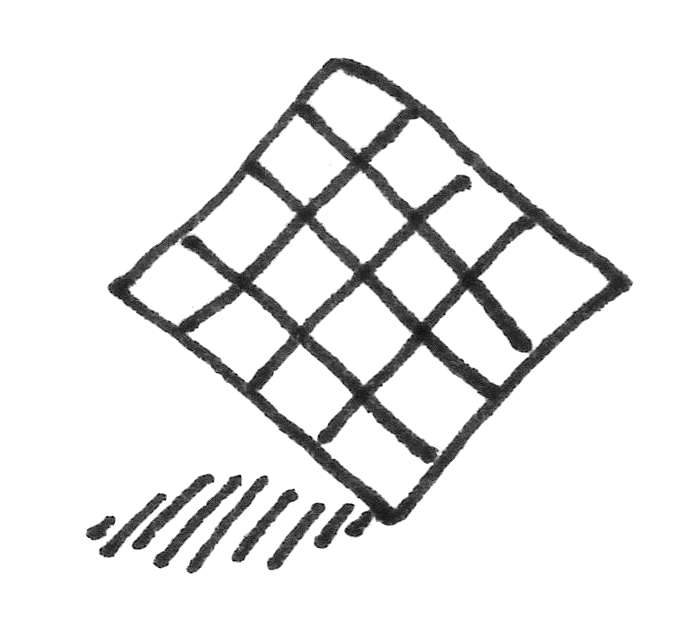
\includegraphics[scale=0.15]{../illustrations/matrix}
\end{center}
\vspace{-2em}
\end{wrapfigure}
\fi

PhyBin~\cite{PhyBin} is a medium-sized (3500-line) bioinformatics
program implemented in Haskell\footnote{Available at
  \url{http://hackage.haskell.org/package/phybin}.} for this purpose,
initially released in 2010.  The primary output of the software is a
hierarchical clustering of the input tree set (that is, a tree of
trees), but most of its computational effort is spent computing an $N
\times N$ distance matrix that records the \emph{edit distance}
between each pair of input trees.  It is this distance computation
that we parallelize in our case study.

\subsection{Computing all-to-all tree edit distance}

The distance metric itself is called \emph{Robinson-Foulds} (RF)
distance, and the fastest algorithm for all-to-all RF distance
computation is Sul and Williams' \emph{HashRF}
algorithm~\shortcite{hashrf}, which is used by a software package of
the same name.\footnote{Available at
  \url{https://code.google.com/p/hashrf/}.}  The HashRF software
package is written in C++ and is about 2-3$\times$ as fast as PhyBin,
which also implements the HashRF algorithm.  Both packages are dozens
or hundreds of times faster than the more widely-used software that
computes RF distance matrices, such as PHYLIP\footnote{Available at
  \url{http://evolution.genetics.washington.edu/phylip.html}.}~\cite{phylip}
and DendroPy\footnote{Available at
  \url{http://pythonhosted.org/DendroPy/}.}~\cite{dendropy}.  These
slower packages use $\frac{N^2-N}{2}$ full applications of the
distance metric, which has poor locality in that it reads all trees in
from memory $\frac{N^2-N}{2}$ times.

To see how the HashRF algorithm improves on this, consider that each
edge in an unrooted phylogenetic tree can be seen as partitioning the
tree's nodes into two disjoint sets, according to the two subtrees
that those nodes would belong to if the edge were deleted.  For
example, if a tree has nodes $\setof{a, b, c, d, e}$, one bipartition
or ``split'' might be $\setof{\setof{a, b}, \setof{c, d, e}}$, while
another might be $\setof{\setof{a, b, c}, \setof{d, e}}$.  A tree can
therefore be encoded as a \emph{set of bipartitions} of its nodes.
Furthermore, once trees are encoded as sets of bipartitions, we can
compute the edit distance between trees (that is, the number of
operations required to transform one tree into the other) by computing
the \emph{symmetric set difference} between sets of bipartitions, and
we can do so using standard set data structures.

\algnewcommand{\LineComment}[1]{\State \(\triangleright\) {#1}\hfill~}

\singlespacing
\begin{algorithm}[t]
  \begin{algorithmic}[0] % 0 means no line numbering
    \LineComment {First phase: populate splits map.}
    \ForAll {$t \in \mathit{alltrees}$}
    \ForAll {$\mathit{bip} \in t$}
    \hspace{3em}\LineComment {Add $t$ to set of trees pointed at by $\mathit{splitsmap}[\mathit{bip}]$,}
    \hspace{3em}\LineComment {adding a key for $\mathit{bip}$ to $\mathit{splitsmap}$ if necessary.}\\
    \hspace{3em}$\mathrm{insert}(t, \mathit{splitsmap}[\mathit{bip}])$
    \EndFor
    \EndFor
    \LineComment {Second phase: populate distance matrix.}
    \LineComment {$\mathrm{values}()$ returns a list of all the values in a dictionary.}
    \ForAll {$\mathit{treeset} \in \mathrm{values}(\mathit{splitsmap})$}
    \ForAll {$t_1 \in \mathit{alltrees}$}
    \ForAll {$t_2 \in \mathit{alltrees}$}
    \If {$t_1 \in \mathit{treeset}$ $\mathrm{XOR}$ $t_2 \in \mathit{treeset}$} \\
    \hspace{6em}$\mathrm{increment}(\mathit{distancematrix}[t_1, t_2])$
    \EndIf
    \EndFor
    \EndFor
    \EndFor
  \end{algorithmic} 
  \caption{Pseudocode of the HashRF algorithm for computing a tree
    edit distance matrix.  $\mathit{alltrees}$, $\mathit{splitsmap}$
    and $\mathit{distancematrix}$ are global variables, defined
    elsewhere.  $\mathit{alltrees}$ is the set of trees, represented
    as sets of bipartitions; $\mathit{splitsmap}$ maps bipartitions to
    sets of trees in which they occur.  In the second phase, the
    comparison of $t_1$ and $t_2$ uses $\mathrm{XOR}$ because the RF
    distance between two trees is defined as the number of
    bipartitions implied by exactly one of the two trees being
    compared.}
  \label{alg:hashrf}
\end{algorithm}
\doublespacing

The HashRF algorithm makes use of this fact and adds a clever trick
that greatly improves locality.  Before computing the actual distances
between trees, it populates a dictionary, the ``splits map'', which maps
each observed bipartition to a set of IDs of trees that contain that
bipartition.  The second phase of the algorithm, which actually
computes the $N \times N$ distance matrix, does so by iterating
through each entry in the splits map.  For each such entry, for each
pair of tree IDs, it checks whether exactly one of those tree IDs is
in the splits map entry, and if so, increments the appropriate
distance matrix entry by one.

Algorithm~\ref{alg:hashrf} is a psuedocode version of the HashRF
algorithm.  The second phase of the algorithm is still $O(N^2)$, but
it only needs to read from the much smaller $\mathit{treeset}$ during
this phase.  All loops in Algorithm~\ref{alg:hashrf} are potentially
parallel.

\subsection{Parallelizing the HashRF algorithm with LVish}

In the original PhyBin source code, the type of the splits map is:

\singlespacing
\begin{lstlisting}
type BipTable = Map DenseLabelSet (Set TreeID)
\end{lstlisting}
\doublespacing

\noindent Here, a @DenseLabelSet@ encodes an individual bipartition as
a bit vector.  PhyBin uses purely functional data structures for the
@Map@ and @Set@ types, whereas the C++ HashRF implementation uses a
mutable hash table.  Yet in both cases, these structures grow
monotonically during execution, making the algorithm a good candidate
for parallelization with LVish.  The splits map created during the
first phase of the algorithm is a map of sets, which can be directly
replaced by their LVar counterparts, and the distance matrix created
in the second phase can be represented as a vector of monotonically
increasing counters.

In fact, the parallel port of PhyBin using LVish was so
straightforward that, after reading the code, parallelizing the first
phase of the algorithm took only 29 minutes.\footnote{Git commit
  range:
  \url{https://github.com/rrnewton/PhyBin/compare/5cbf7d26c07a...6a05cfab490a7a}.}
Tables~\ref{t:phybin-bench} and~\ref{t:phybin-bench-hashrf} show the
results of a running time comparison of the parallelized PhyBin with
DendroPy, PHYLIP, and HashRF.  We first benchmarked PhyBin against
DendroPy and PHYLIP using a set of 100 trees with 150 leaves each.
Table~\ref{t:phybin-bench} shows the time it took in each case to fill
in the all-to-all tree edit distance matrix and get an answer back.
PhyBin was much faster than the two alternatives.

\begin{table}
\begin{tabularx}{.75\textwidth}{XXXXX}
Trees & Species & DendroPy & PHYLIP & PhyBin    \\ \hline
100   & 150     & 22.1s    & 12.8s  & \textbf{0.269s}
\end{tabularx}
\caption{PhyBin performance comparison with DendroPy and PHYLIP.}
\label{t:phybin-bench}
\end{table}

\begin{table}
\begin{tabularx}{\textwidth}{XXXXXXX}
\multirow{2}{*}{Trees} & \multirow{2}{*}{Species} & \multirow{2}{*}{HashRF} & \multicolumn{4}{c}{PhyBin}                \\
                       &                          &                         & 1 core & 2 cores & 4 cores & 8 cores      \\ \hline
1000                   & 150                      & \textbf{1.7s}           & 4.7s   & 3.0s    & 1.9s    & \textbf{1.4s}
\end{tabularx}
\caption{PhyBin performance comparison with HashRF.}
\label{t:phybin-bench-hashrf}
\end{table}

Then, to compare PhyBin with HashRF, we used a set of 1000 trees with
150 leaves each.  Table~\ref{t:phybin-bench-hashrf} shows the results.
HashRF took about 1.7 seconds to process the 1000 trees, but since it
is a single-threaded program, adding cores does not offer any speedup.
PhyBin, while slower than HashRF on one core, taking about 4.7
seconds, speeds up as we add cores and eventually overtakes HashRF,
running in about 1.4 seconds on 8 cores.  Therefore LVish gives us a
parallel speedup of about $3.35\times$ on 8 cores.  This is exactly
the sort of situation in which we would like to use LVish---to achieve
modest speedups for modest effort, in programs with complex data
structures (and high allocation rates), and without changing the
determinism guarantee of the original functional code.
